\documentclass{beamer}
%\documentclass[handout]{beamer}

\mode<presentation>{
  \usetheme{Warsaw}
  \setbeamercovered{transparent}
}

\mode<handout>{
  \usepackage{pgfpages}
  \pgfpagesuselayout{4 on 1}[a4paper,border shrink=5mm,landscape]
  \setbeamercolor{background canvas}{bg=black!5}
}

\usepackage[english]{babel}
\usepackage[latin1]{inputenc}
%\usepackage{times}
%\usepackage[T1]{fontenc}
\usepackage{tikz}
\usepackage{graphicx}
%\usepackage{hyperref}
%\include{pythonlisting}
\usepackage{url}
\usepackage{caption}
\usepackage{subcaption}
\usepackage{float}

\usepackage{colortbl}
\usepackage{color}

%\cellcolor[rgb]{1,0,0} 6

\useoutertheme[subsections=false]{smoothbars}

\title[Metropolis and Wang-Landau algorithms]{A Comparison of the Metropolis and Wang-Landau Algorithms Applied to the Potts Model}

\author{Gwylim Ashley}

\date{24 October 2012}

\AtBeginSection[]{
  \begin{frame}<beamer>{Outline}
    \tableofcontents[currentsection,currentsubsection]
  \end{frame}
}

\begin{document}

\begin{frame}
  \titlepage
\end{frame}

\section{Background}
\begin{frame}{Random walks}
    \begin{itemize}
        \item Statistical mechanics: to obtain an average variable $\langle X\rangle$ for a system, calculate $\frac{1}{Z}\sum_s X(s)e^{-\beta E(s)}$.
        \item Number of microstates $s$ is too large to directly sum - how can we choose a representative sample of microstates?
        \item We use a \emph{Monte-Carlo method}, in particular, a \emph{random walk} - we choose an arbitrary initial microstate and make incremental changes according to some (randomized) algorithm.
    \end{itemize}
\end{frame}
\begin{frame}{The Potts model}
    \begin{itemize}
        \item The Potts model is a simple example to study, having a first-order phase transition.
        \item Consists of an $l\times l$ lattice of particles, each having a ``spin'' $s \in \{0,...,q-1\}$.
        \item Particles interact only with nearest neighbors, $H = \sum_{v, w\text{ adjacent}}(1 - \delta(s_v, s_w))$.
        \item Predicted phase transition at $\beta = \log(1 + \sqrt q)$.
    \end{itemize}
\end{frame}
\begin{frame}{Metropolis algorithm}
    \begin{itemize}
        \item The Metropolis algorithm estimates a Boltzmann distribution at a particular temperature $T = 1/\beta$.
        \item We perform the random walk by starting at a vertex $v$ and going to an adjacent vertex $w$ with probability $min\{1, e^{\beta(E(v) - E(w))}\}$.
        \item After some number of steps, the current vertex will be a suitable sample from the Boltzmann distribution.
    \end{itemize}
\end{frame}
\begin{frame}{Wang-Landau algorithm}
    \begin{itemize}
        \item A more complicated algorithm which calculates the density of states $g(E)$.
        \item Instead of using a ratio of Boltzmann factors, we use $g(E(v))/g(E(w))$.
        \item Increase $g(E)$ whenever we visit energy level $E$.
        \item When algorithm converges, we obtain a flat histogram over $E$, and a good estimate of $g(E)$.
    \end{itemize}
\end{frame}
\section{Results}
\begin{frame}{Convergence}
    \begin{figure}[H]
        \begin{subfigure}[t]{1.5in}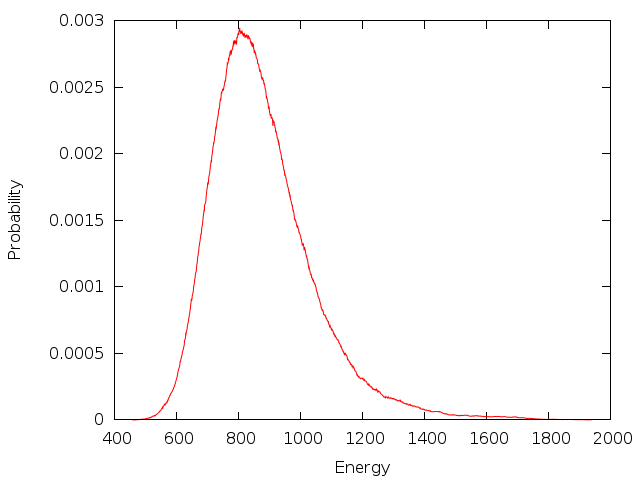
\includegraphics[width=1.5in]{../results/metropolis/m50.png}\caption{Metropolis}\end{subfigure}
        \begin{subfigure}[t]{1.5in}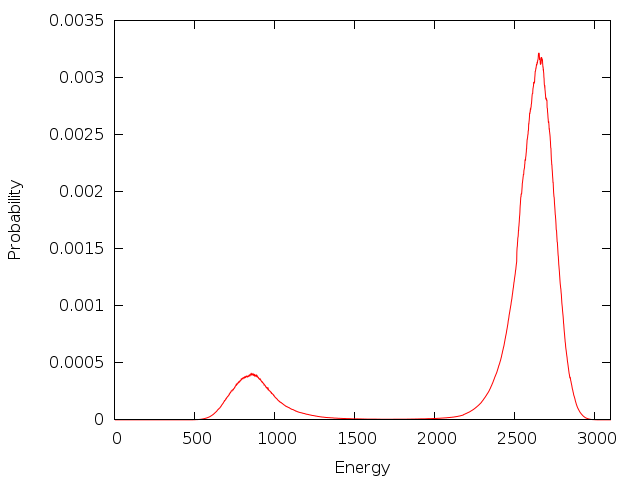
\includegraphics[width=1.5in]{../results/wanglandau/b50.png}\caption{Wang-Landau}\end{subfigure}
        \caption{Obtained Boltzmann distribution for $l = 50$, $\beta = 1.424$}
    \end{figure}
    \begin{itemize}
        \item Due to the structure of the Boltzmann distribution at transition temperature, the Metropolis algorithm has slow convergence here.
        \item For $l = 30$, same result obtained for Metropolis and Wang-Landau, for $l = 50$, results as above are obtained.
    \end{itemize}
\end{frame}
\begin{frame}{Derived quantities}
    \begin{figure}[H]
        \begin{subfigure}[t]{1.5in}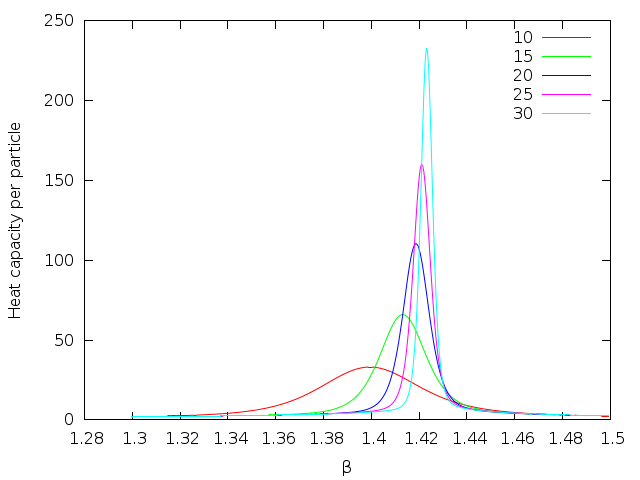
\includegraphics[width=1.5in]{../results/wanglandau/capacity.png}\caption{Heat capacity as a function of $l$}\end{subfigure}
        \begin{subfigure}[t]{1.5in}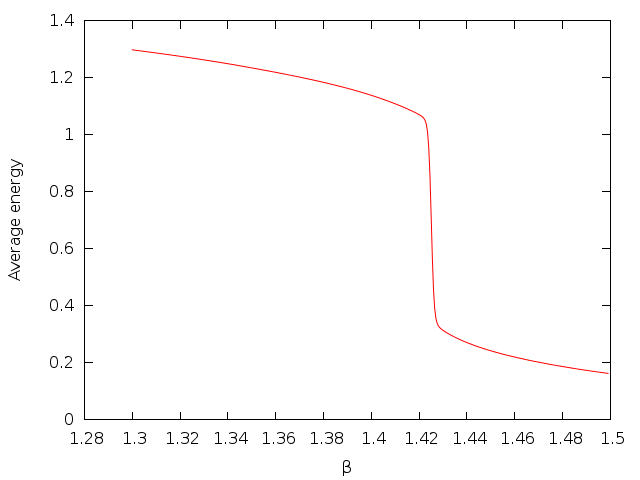
\includegraphics[width=1.5in]{../results/wanglandau/e50.png}\caption{Energy as a function of $\beta$ for $l = 50$}\end{subfigure}
        \caption{Derived quantities from density of states}
    \end{figure}
    \begin{itemize}
        \item We can calculate the heat capacity $C = \beta^2\left(\langle E^2\rangle - \langle E\rangle^2\right)$ and the average energy $\langle E\rangle$ as a function of temperature.
        \item Results consistent with theory. Phase transition is sharper for larger $l$.
    \end{itemize}
\end{frame}
\section{Conclusion}
\begin{frame}{Conclusion}
    \begin{itemize}
        \item Monte-Carlo techniques are useful for dealing with large systems that can't be handled directly.
        \item For some systems, the Metropolis algorithm has slow convergence. Wang-Landau avoids this.
        \item An estimate of the density of states $g(E)$ is useful for deriving other quantities.
    \end{itemize}
\end{frame}

\end{document}
